%!TEX root=paper.tex

% \newpage
\section{A Minimum Viable Language Textbook}
\label{sec:system}

Our long term vision, of an ecosystem where various educational applications, created by different authors, interacting and sharing information in order to maximize the efficiency and enjoyment of the vocabulary improvement process is described in more detail elsewhere \cite{Lungu16}. 

Figure \ref{fig:architecture} highlights two types of applications that are relevant for implementing a language textbook: the {\bf interactive reader apps} allow the learners to interact with texts in their preferred context (e.g. eBooks, News, Blogs), and the {\bf vocabulary trainer apps} allow the readers to practice vocabulary exercises. 
% 
The figure also presents several critical components of the ecosystem with which the applications interact: the learner model, the translation service, the content recommender, and vocabulary recommender. Before we convince other system creators to join such an ecosystem, we have decided to build a {\em minimum viable ecosystem} which includes basic implementations of the core components. In this section we briefly describe the various back-end components, and in the next we describe the user interface of a unified, web-based reader and trainer app. 

\begin{figure}[h!]
\centering
  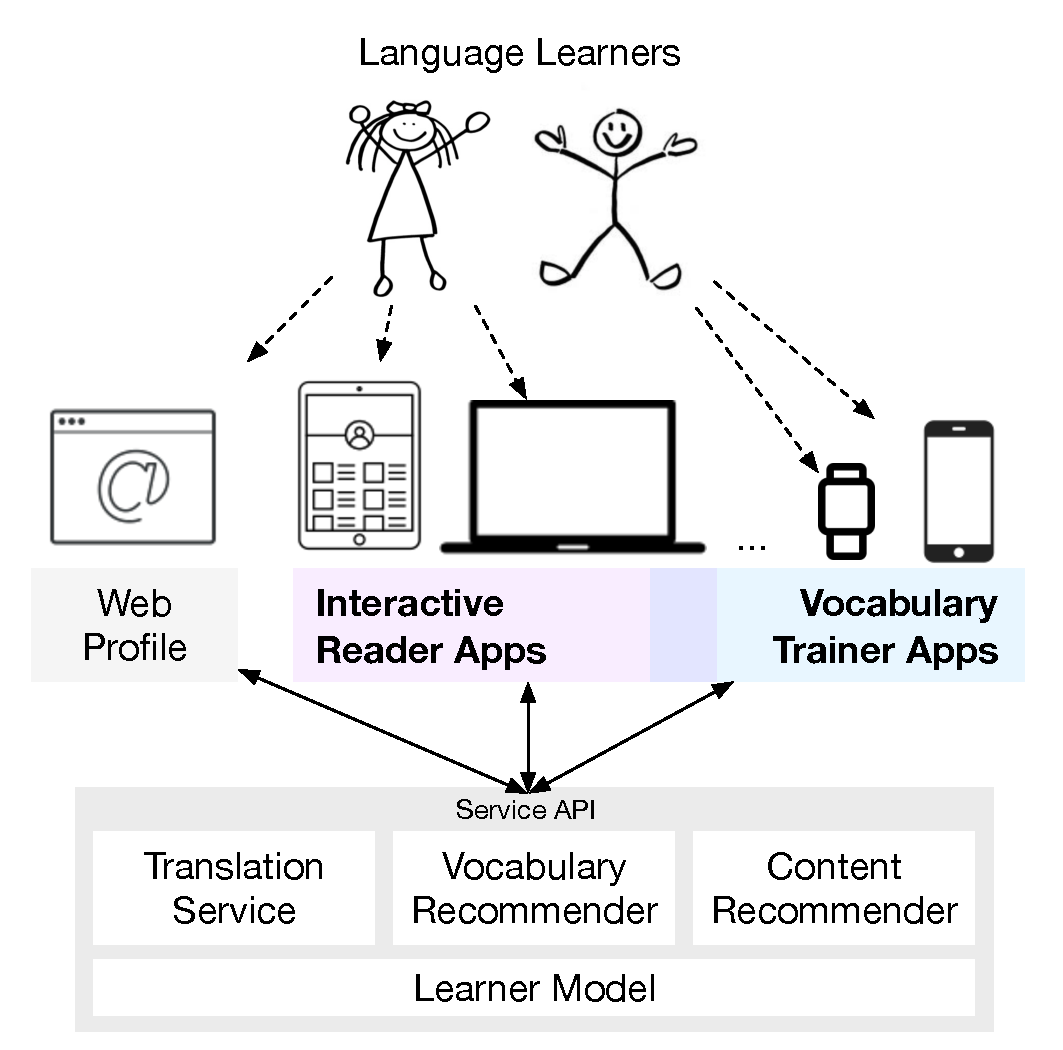
\includegraphics[width=0.7\columnwidth]{figures/zeeguu-architecture.pdf}
  \caption{The architecture of the envisioned software ecosystem}~\label{fig:architecture}
\end{figure}

\subsection{Learner Model}

At the core of the ecosystem a ``learner model'' tracks the evolving knowledge of the learner. 
Based on the learner model, algorithms can make recommendations for the individual applications regarding interesting content to read and appropriate vocabulary to study. The individual applications, in turn, report back to the learner model events from which the learner progress can be infered. 

Currently, the model tracks the probabilities of a user knowing words based on interaction events in the apps: asking for a translation, repeatedly encountering a given word without asking for a translation, or answering an vocabulary exercise.


\subsection{The Translation Service}

The Translation Service is a subsystem implemented using Python which provides translations to all the applications in the ecosystem. Instead of implementing our own contextual translation engine, we rely on existing industrial grade translation APIs. To avoid depending on a single service and to also increase the likelihood that at least one of the alternative translations is the correct one, the translation service dispatches in parallel requests to at least three third party translation APIs: Google Translate, Microsoft Translate, and Glosbe. \cite{Jager17-mux} The first two provide contextual translations and multi-word translations, while the third is a simple dictionary. 

The dependency of the translation service on multiple third party APIs allows for a higher reliability and a chance to guarantee a low response time: when a service is down or too slow to respond, the results from it are ignored. We detail elsewhere the strategies we use to keep response times low\cite{Jager17-mux}.

It is critical that the translation service be used by all the applications in the ecosystem since this allows the server to track the words and the context in which they are being looked up. This information is then used for estimating learner knowledge and for generating personalized recommendations. 


% by interacting with a core API that provides the basic contextual translations, user knowledge estimation, and recommendations for words to be studied and texts to be read \cite{Lungu16}. 

\subsection{Vocabulary Recommender}

The goal of the vocabulary recommender is to program optimally-timed words to practice. 

To schedule the words to practice the system uses an adaptive, response-time-based scheduling algorithm [was developed] to increase the efficiency of perceptual learning by Mettler et al. \cite{Mettler14-ARTS}. After evaluating several alternative scheduling strategies we settled on the Mettler one since it has been proven to have gains with both familiar, seen items as well as with new, unseen instances and the benefits of adaptive scheduling were present at an immediate test as well as at a delay \cite{Mettler14-ARTS}.


\subsection{Content Recommender}

The content recommender aims to present the reader with texts that are both interesting and accessible at the same time.

The current implementation of the text recommender allows the reader to select online sources (e.g. news, blogs) that are interesting for them. The sources are scanned for the latest articles and cached by using a custom-made library\footnote{The library called {\em watchmen} is open sourced at:\\ https://github.com/zeeguu-ecosystem/watchmen}. 
% The user interface for the article selection is presented in the next section. 

Currently, the difficulty of a text is computed by aggregating the individual difficulty of the words it contains. The individual word difficulty, which can vary from 0 to 10, and is computed in the following way: 
% taking into account the ranking of words in the target language based on frequency combined with the past history of a given user's activity: 

\begin{itemize}
	\item When the word is estimated to be known, its difficulty is considered to be zero. The word can be known either based on past readings (i.e. encountered multiple times, but never looked up) or based on past vocabulary exercises (i.e. correctly identified in the most recent exercises) 
	\item When the word is in the top 50K most frequent words in the target language, it's difficulty is 	considered to increase with 0.1 for every 500 words; if the word is not in top 50K, its difficulty is ten.
\end{itemize}

With these strategies for computing word difficulty, the text difficulty is computed as the median of the words in the text. 
% In the future we plan to investigate other measures.  


\newpage
\section{A Web-Based Reader and Trainer Platform}
% as we is composed of instantiations of the components. We present them in turn in this section, focusing the discussion on three key activities that a user of such an interactive textbook is interested in: 

% \begin{enumerate}
	% \item finding texts to read
	% \item reading the found texts
	% \item practicing vocabulary in context
% \end{enumerate}

 % interacts with: the reader and the trainer applications. 
% \begin{added}
	
	In this section we present the user interface of the prototype {\em personalized language textbook} that we have built. It combines in a single responsive web application a reader applications and a voabulary trainer with multiple exercise types, and thus, can be used from a variety of devices. In the experiments reported in this paper, it was used from Windows, Android, and iOS devices. Although not presented here, since it was not used in the experiments, a smartwatch application also exists as another vocabulary trainer.

% \end{added}




%!TEX root=paper.tex

% \newpage
% \subsection{Web Article Reader}


    % A basic text reader should allow the learners to find interesting texts (e.g. news, blogs) and should provide a facile interaction for reading and translating unknown words. 
  
% The Web Article Reader allows the learners to subscribe to various sources of articles (e.g. news, blogs) and provides a facile interaction for reading and translating unknown words. 
% It consists of several components:

\subsection{Finding Personally Interesting and Accessible Texts}
% personally relevant vs. interesting... relevant can mean both interesting and not too difficult. 
% \ml{make sure that we use source consistently in the text; not feed for example.}
% From the user's point of view, the Reader is organized around {\em sources\xspace} of articles. The system categorizes sources by their language. 
The current system allows the learners to subscribe to various online sources (i.e. news, blogs) and then monitors those sources for new texts. Figure \ref{fig:system_subscriptions} presents the source subscription dialog listing multiple text sources for French.
% multiple sources for every language are pre-loaded in the system and if a reader wants to add a new source they have to send an email to the maintainers of the system. 



    \begin{figure}[h!]
    \centering
      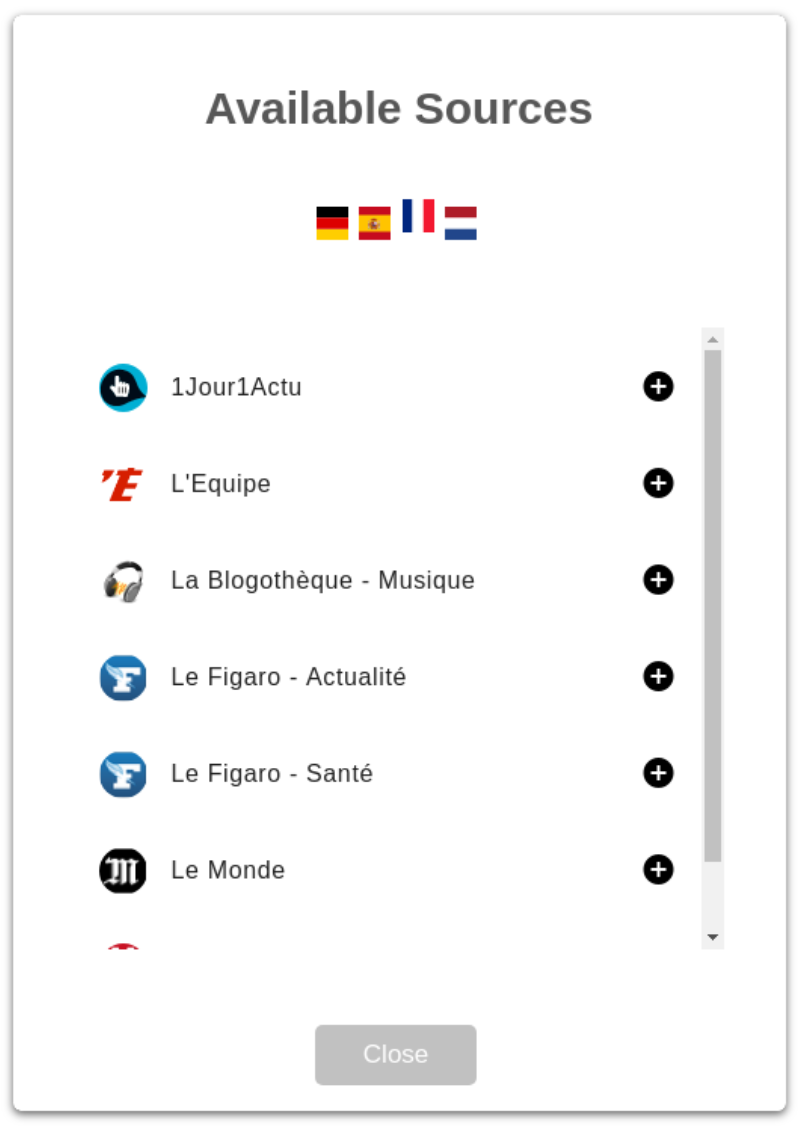
\includegraphics[width=0.3\columnwidth]{figures/available_sources}
      \caption{Different users subscribe to different sources}~\label{fig:system_subscriptions}
    \end{figure}

% A multi-lingual learner can subscribe to multiple sources in different languages. 
% \begin{added}

  Once a reader is subscribed to a source, that source is constantly monitored for new articles, which are recommended to the learner in an article browser like the one in Figure \ref{fig:article_listing}. The browser displays for each article an icon representing its source, a title, a summary, and an estimated difficulty level.
  To visualize the reading difficulty of an article, there are three levels of information displayed: 1) a flag representing the language of the article since a learner could be actually registered to feeds in multiple languages; 2) a color coded difficulty from green to yellow to red, to  allow the user to rapidly judge difficulty on an intuitive level; 3) a numerical difficulty score  to allow a more quantitative judgment of the estimated difficulty.
    
% \end{added}

    \begin{figure}[h!]
    \centering
      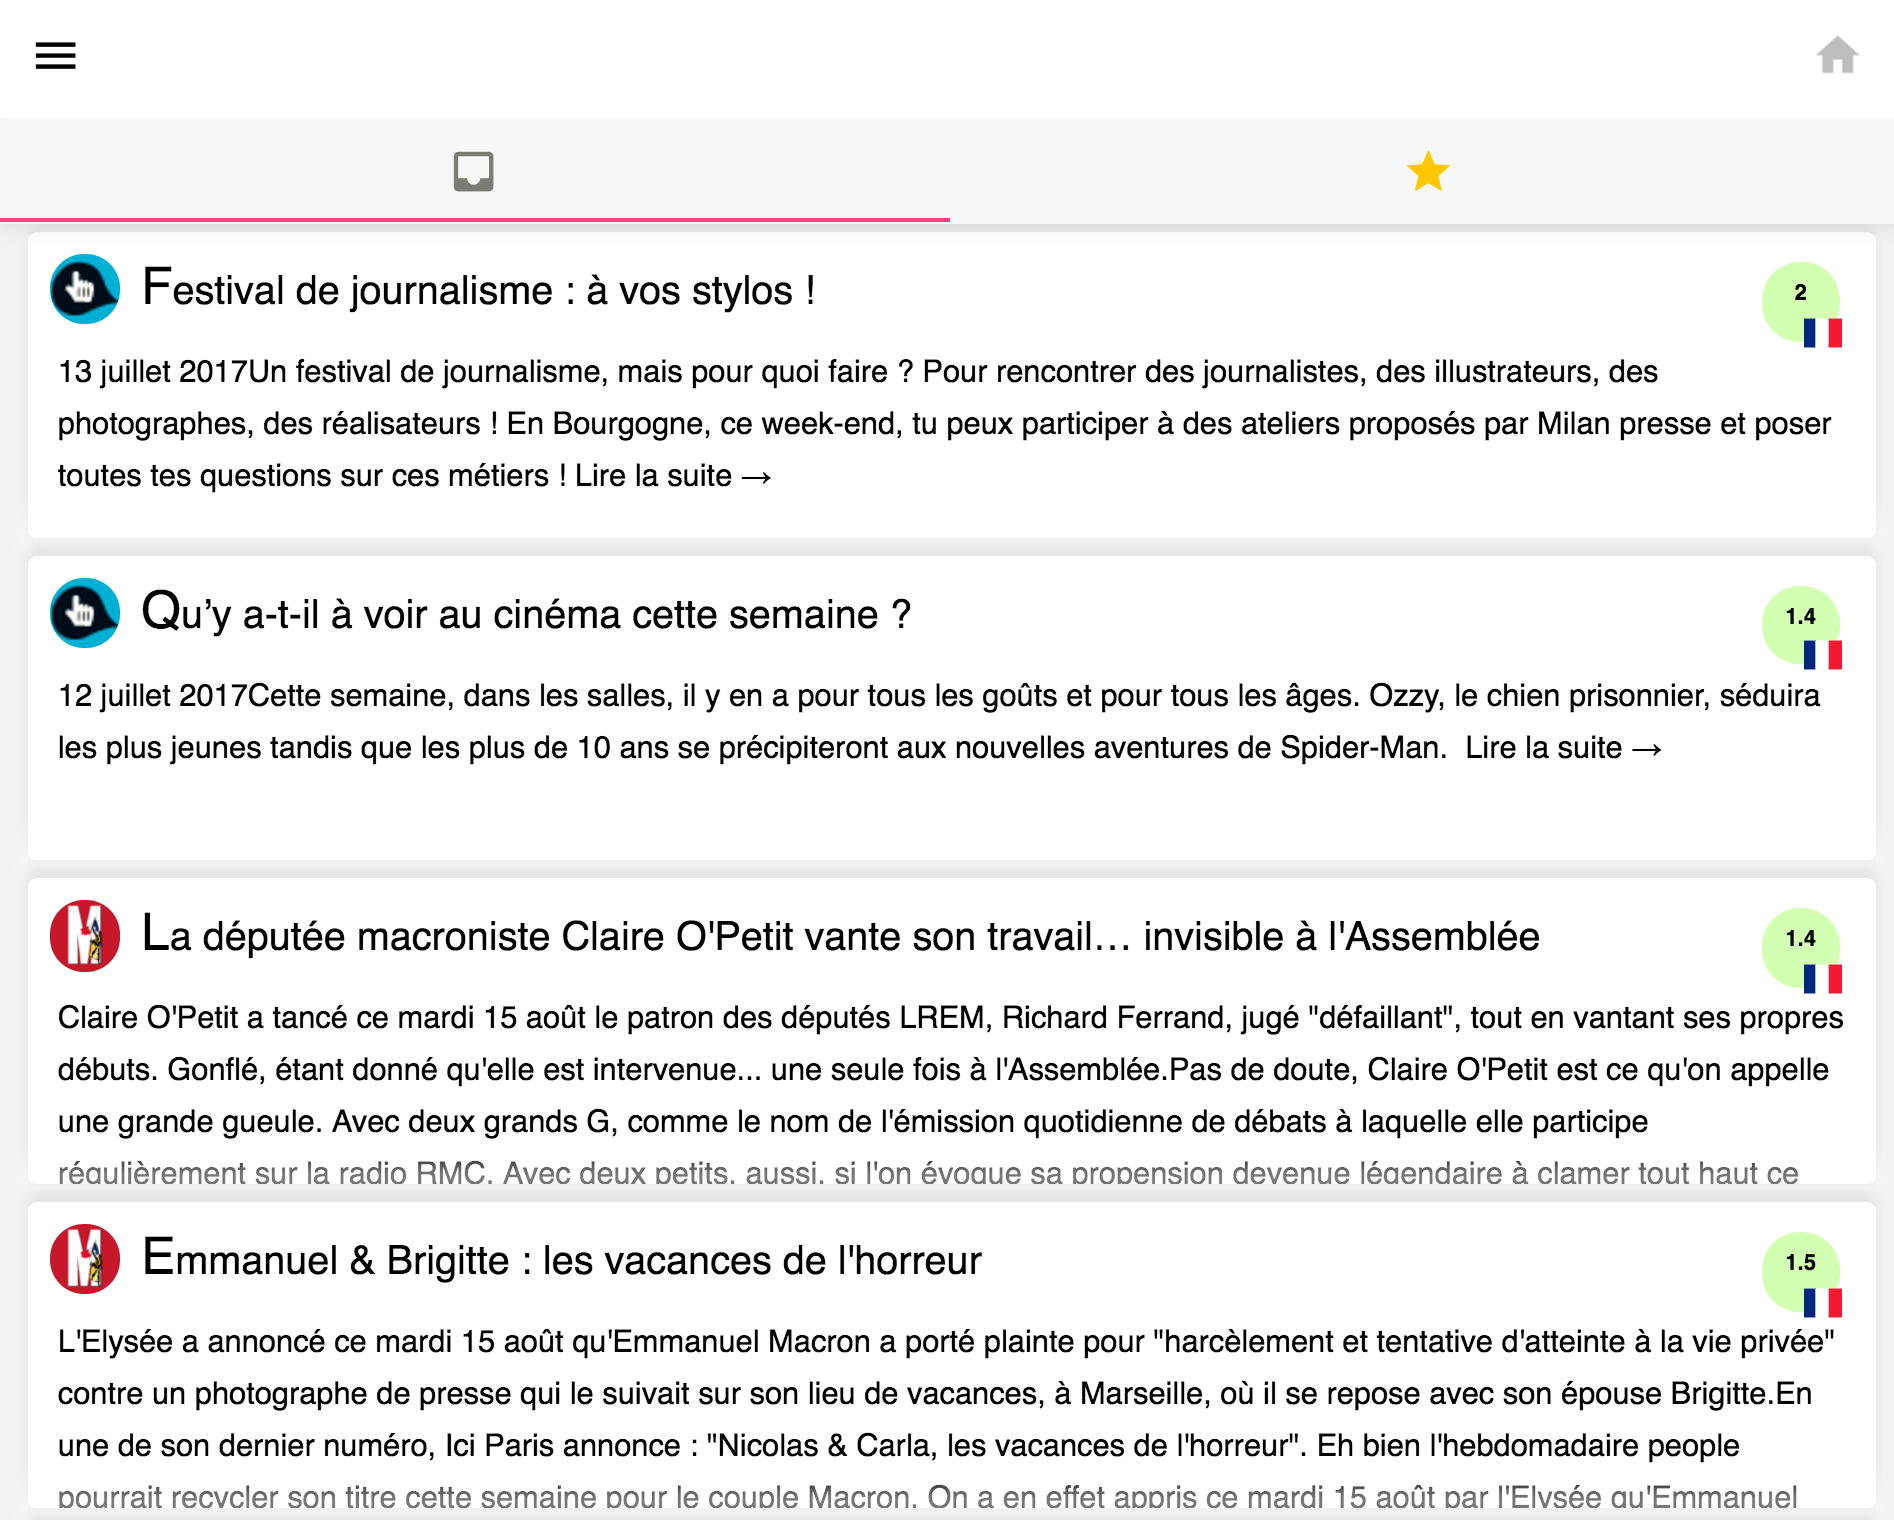
\includegraphics[width=0.75\columnwidth]{figures/article_listing}
      \caption{Article listing presents estimated difficulty levels }~
      \label{fig:article_listing}
    \end{figure}



Difficulty estimation takes into account the frequency of the vocabulary items in the text. The system filters out articles that are too difficult given that it was deployed with non-advanced learners.\footnote{This is one of the limitations of the system that we discuss later.}

\subsection{Interacting With Unknown Words While Reading}
% Reading Texts to Understand

To make reading as facile as possible, the reader is optimized for the most frequent action that a reader is likely to want to perform: translating a word. Thus, when a user clicks on a word, a translation is inserted right after the word, as Figure \ref{fig:translated_word} illustrates: 

\begin{figure}[h!]
\centering
  
\includegraphics[width=0.7\columnwidth]{figures/translated_word}
  \caption{A translated word is inserted after the tapped word.}~\label{fig:translated_word}
\end{figure}

Two other alternatives that we explored and eventually dropped (for each had disadvantages) were: 

\begin{enumerate}

  \item Temporarily showing a popup of the translation and then hiding it again. This had a disadvantage for difficult sentences, where multiple words must be translated. The reader can forget translated words by the time they arrive at the end of an article, requiring them to re-translate.
  \item Using the native selection mechanism to select text as opposed to click / touch. 
  % We experimented with allowing the learner to select a word in the same way this is normally done on the corresponding platform. 
  This had the disadvantage that native selection is not designed as a priority action and thus is slow to respond (e.g. on Android a user must hold their fingertip down for almost a second before the contextual menu is displayed). 
\end{enumerate}


\subsubsection{Translating Multi-Word Expressions}

The user can chain a few consecutive words into a single translation by simply tapping adjacent words which are then automatically merged in a translation bubble (Figure \ref{fig:translation_extension}). This is useful for collocations and in cases where by expanding the translated set of words the precision of the translation increases. 

    \begin{figure}[h!]
    \centering
      
\includegraphics[width=0.7\columnwidth]{figures/translated_words1}
      
\includegraphics[width=0.7\columnwidth]{figures/translated_words2}
      \caption{When adjacent words are tapped the translation bubble is extended accordingly}~\label{fig:translation_extension}
    \end{figure}

This minimalistic interaction model serves a double purpose - it enables and eases the translation of several chained words but it discourages users from translating entire sentences or phrases. This is in line with the recommendations of the literature (e.g. Renandya argues that extensive reading should discourage intensive use of translations\cite{renadya07-power}) but also because it reduces the amount of characters which are being translated by the learner (and thus the costs of the system, since some of the translation services have a per-character fee). 

One of the limitations of this interaction is that it is not clear (at least at the moment) how to expand it for the situations in which expressions are present that are composed of words which are not adjacent (e.g. particle verbs in German).


\subsubsection{Compensating for the Limits of Machine Translation}
Due to the limitations of machine translation multiple translations might be possible in a given context. In such a case the system will insert the most likely alternative as described earlier right after the selected text, but it will allow the reader to discover alternatives. With a click on the translation, a drop-down menu appears in which alternatives are presented. Figure \ref{fig:registrations} shows that besides the predefined alternatives the learner can provide their own translation via an input box (the third line, ``took place'' is typed in by the learner in the figure). 


\begin{figure}[h!]
\centering
  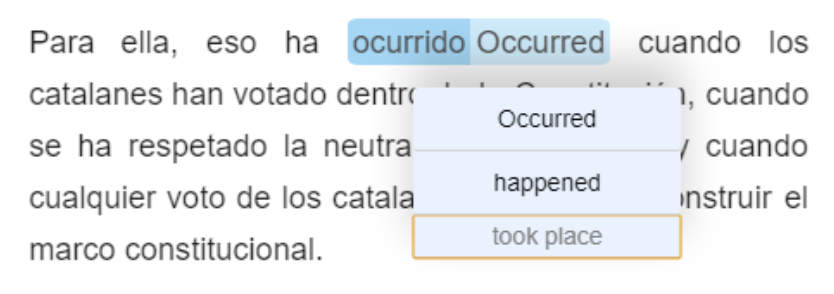
\includegraphics[width=0.7\columnwidth]{figures/translation_alter_menu}
  \caption{A translated word is inserted after the tapped word.}~\label{fig:registrations}
\end{figure}

\subsubsection{Discovering the Pronounciation of a Word}

The process we followed while developing the reader was an iterative process, with short release cycles (one or two weeks), and frequent testing with members of the research team, and the occasional external user. 

One of the features that we added following a suggestion of an early beta-tester -- a teacher of Dutch as a foreign -- was the pronounciation of a translated word. After exploring several trade-offs between flexibility, ease of use, and a clean user interface, we settled on triggering the pronounciation of a word (or group of words) with a tap. 

% The pronounciation is generated by using the HTML5 Speech API which is supported by most modern browsers both on the mobile and on the desktop. 

% \ml{could ask the users if they are happy with it.}
% Although no user has yet complained about it, this means that a user can not pronounce a word without it being translated first. It might also be that for some languages this is more important than for others, and we just did not have users learning those languages (e.g. Danish is notoriously hard to pronounce). In the future we plan to expand the interaction modes to allow pronounciation to exist seperately from translation.
%!TEX root=paper.tex

\newpage
\subsection{Web Vocabulary Trainer}

Given the list of words that a user does not know since they were looked  up in the past we can generate exercises for they user.

Figure \ref{exercise_translate} shows such a generated exercise which asks the reader to translate a given word in the context in which it was encountered in a past reading. The main interactive elements (IEs) that are specific to this exercise are an input box that allows the user to enter a solution (IE5); a button for checking the correctness of the input answer (IE2); a hint button which presents the correct answer (IE1). Two types of control that span exercise types are: a word pronunciation option (IE3) and a feedback option (IE4) which allows the user to provide feebdack about the exercise.

\begin{figure}[h!]
\centering
  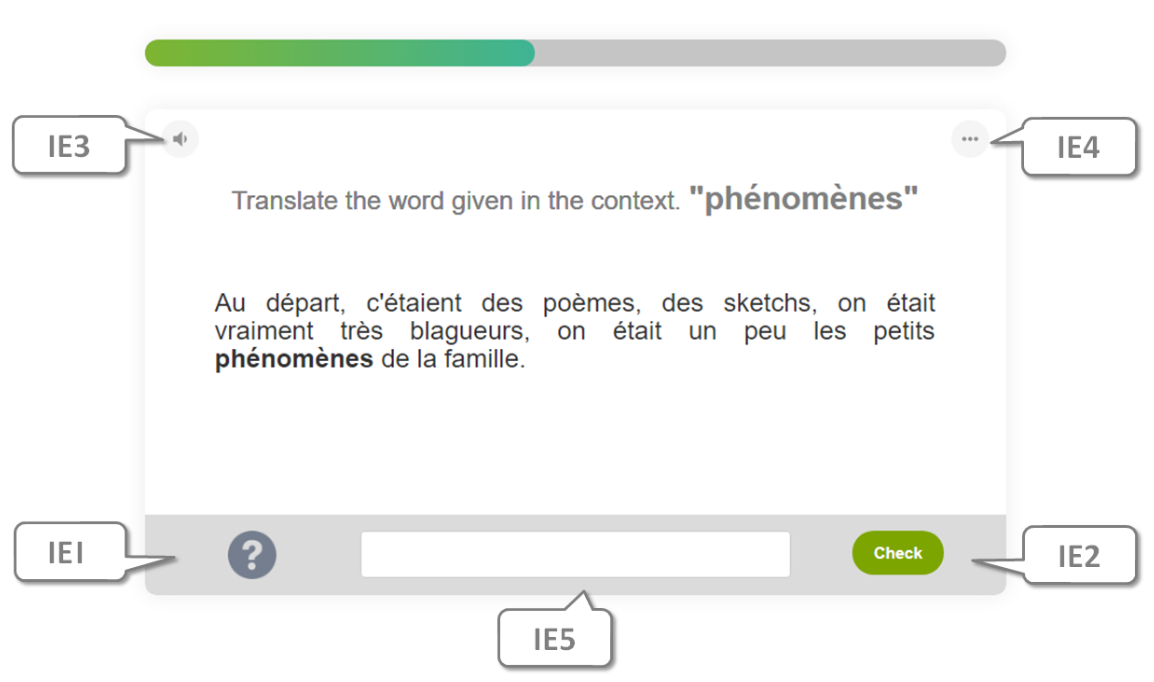
\includegraphics[width=0.9\columnwidth]{figures/exercise_translate}
  \caption{One of the exercise types with which the user is presented asks the user to translate a word in a context that is retrieved from the user's past readings}{
  \label{exercise_translate}
  }
\end{figure}

\ml{The system currently implements three other types of vocabulary practice exercises: one similar to the one in figure, but where the user has to select one of three possible translations, one where the user has to translate to the learned language, not to his known language. A third type of exericse asks the learner to match translations to originals}.

\subsubsection{Selecting Words to Study}

Since a learner might encounter many words that are not understood, we need to prioritize those that are to be studied in exercises. We use three aspects to prioritize words: 

% The words good for study are the ones that are either starred by the user, or are important and of quality based on a set of heuristics. 

\begin{description}

  \item [Important Words] are the ones which appear frequently in the language. For word frequencies we use frequencies computed based on movie subtitles which have been shown to be highly representative to frequencies in human interacitons \cite{New07-subtitles}. 
  
  \item [Quality Context] we favor words that come with a context which is not too short but not too long. 

\end{description}

\subsection{Study Recommender}

The scheduling algorithm is based on an adaptive, response-time-based scheduling algorithm [was developed] to increase the efficiency of perceptual learning by Mettler et al. \cite{Mettler14-ARTS}. After evaluating several alternative scheduling strategies we settled on the Mettler one since it has been proven to have gains with both familiar, seen items as well as with new, unseen instances and the benefits of adaptive scheduling were present at an immediate test as well as at a delay \cite{Mettler14-ARTS}.



% \subsection{Translator Service}

% The core API of the ecosystem provides translations. The main advantage of this indirection is that this allows the server to track the words that are looked up and the context (sentence) in which they are being looked up. This information is then used for estimating learner knowledge and for generating personalized exercises. 

% The Translation Service is an API implemented using Python. Instead of implementing our own contextual translation engine, we decided to rely on existing industrial grade translation APIs. To avoid depending on a single service and to also increase the likelihood that at least one of the alternative translations is the correct one, the translation service dispatches in parallel requests to at least three third party translation APIs: Google Translate, Microsoft Translate, and Glosbe. \cite{Jager17-mux} The first two provide contextual translations and multi-word translations, while the third is a simple dictionary. 

% The dependency of the translation service on multiple third party APIs allows for a higher reliability and a chance to guarantee a low response time: when a service is down or too slow to respond, the results from it are ignored. We detail elsewhere the strategies we use to keep response times low\cite{Jager17-mux}.


% \begin{figure}[h!]
% \centering
%   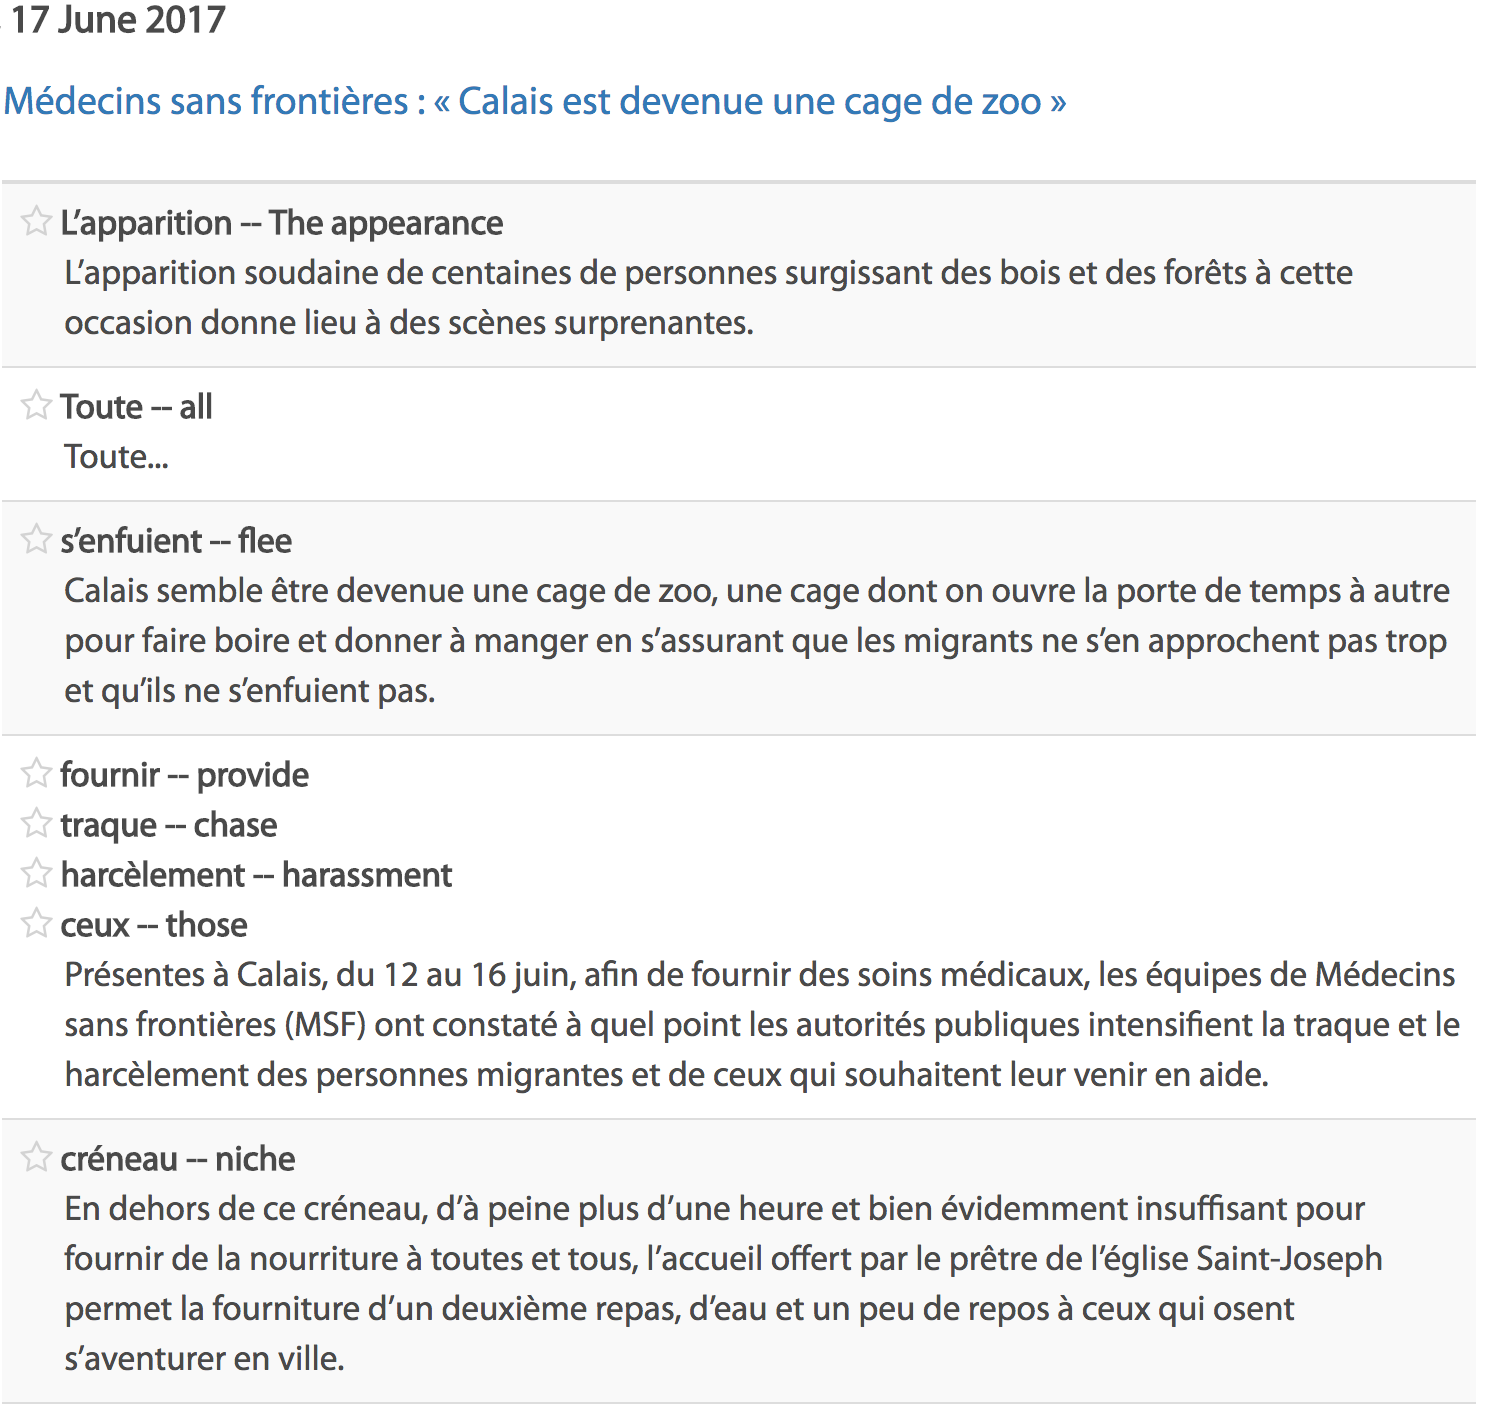
\includegraphics[width=\columnwidth]{figures/teacher_dashboard.png}
%   \caption{A teacher can see the log of the words that a student looked up, their chosen translations, and the corresponding contexts}{
%   \label{fig:teacher}
%   }
% \end{figure}




